\begin{figure*}[t!]
\centerline{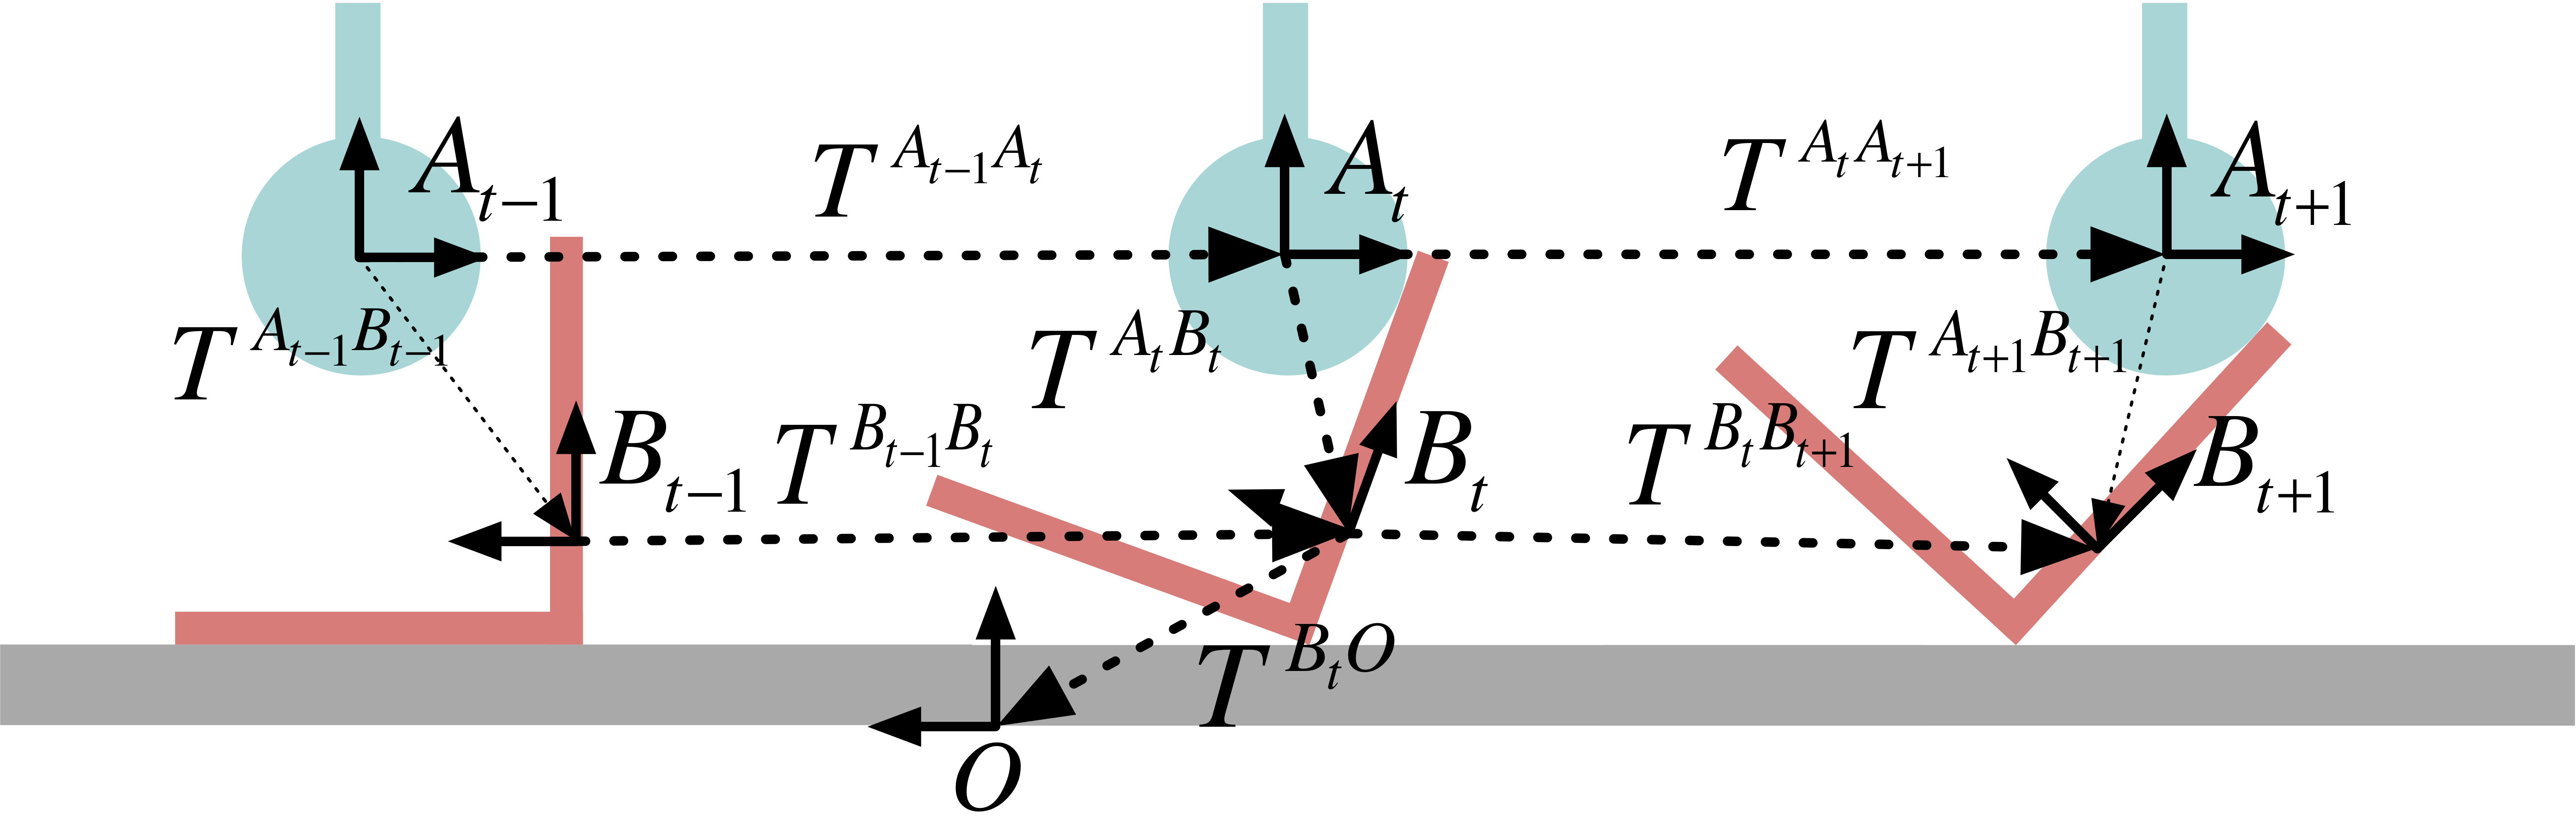
\includegraphics[width=0.67\textwidth]{sequential-frames}
%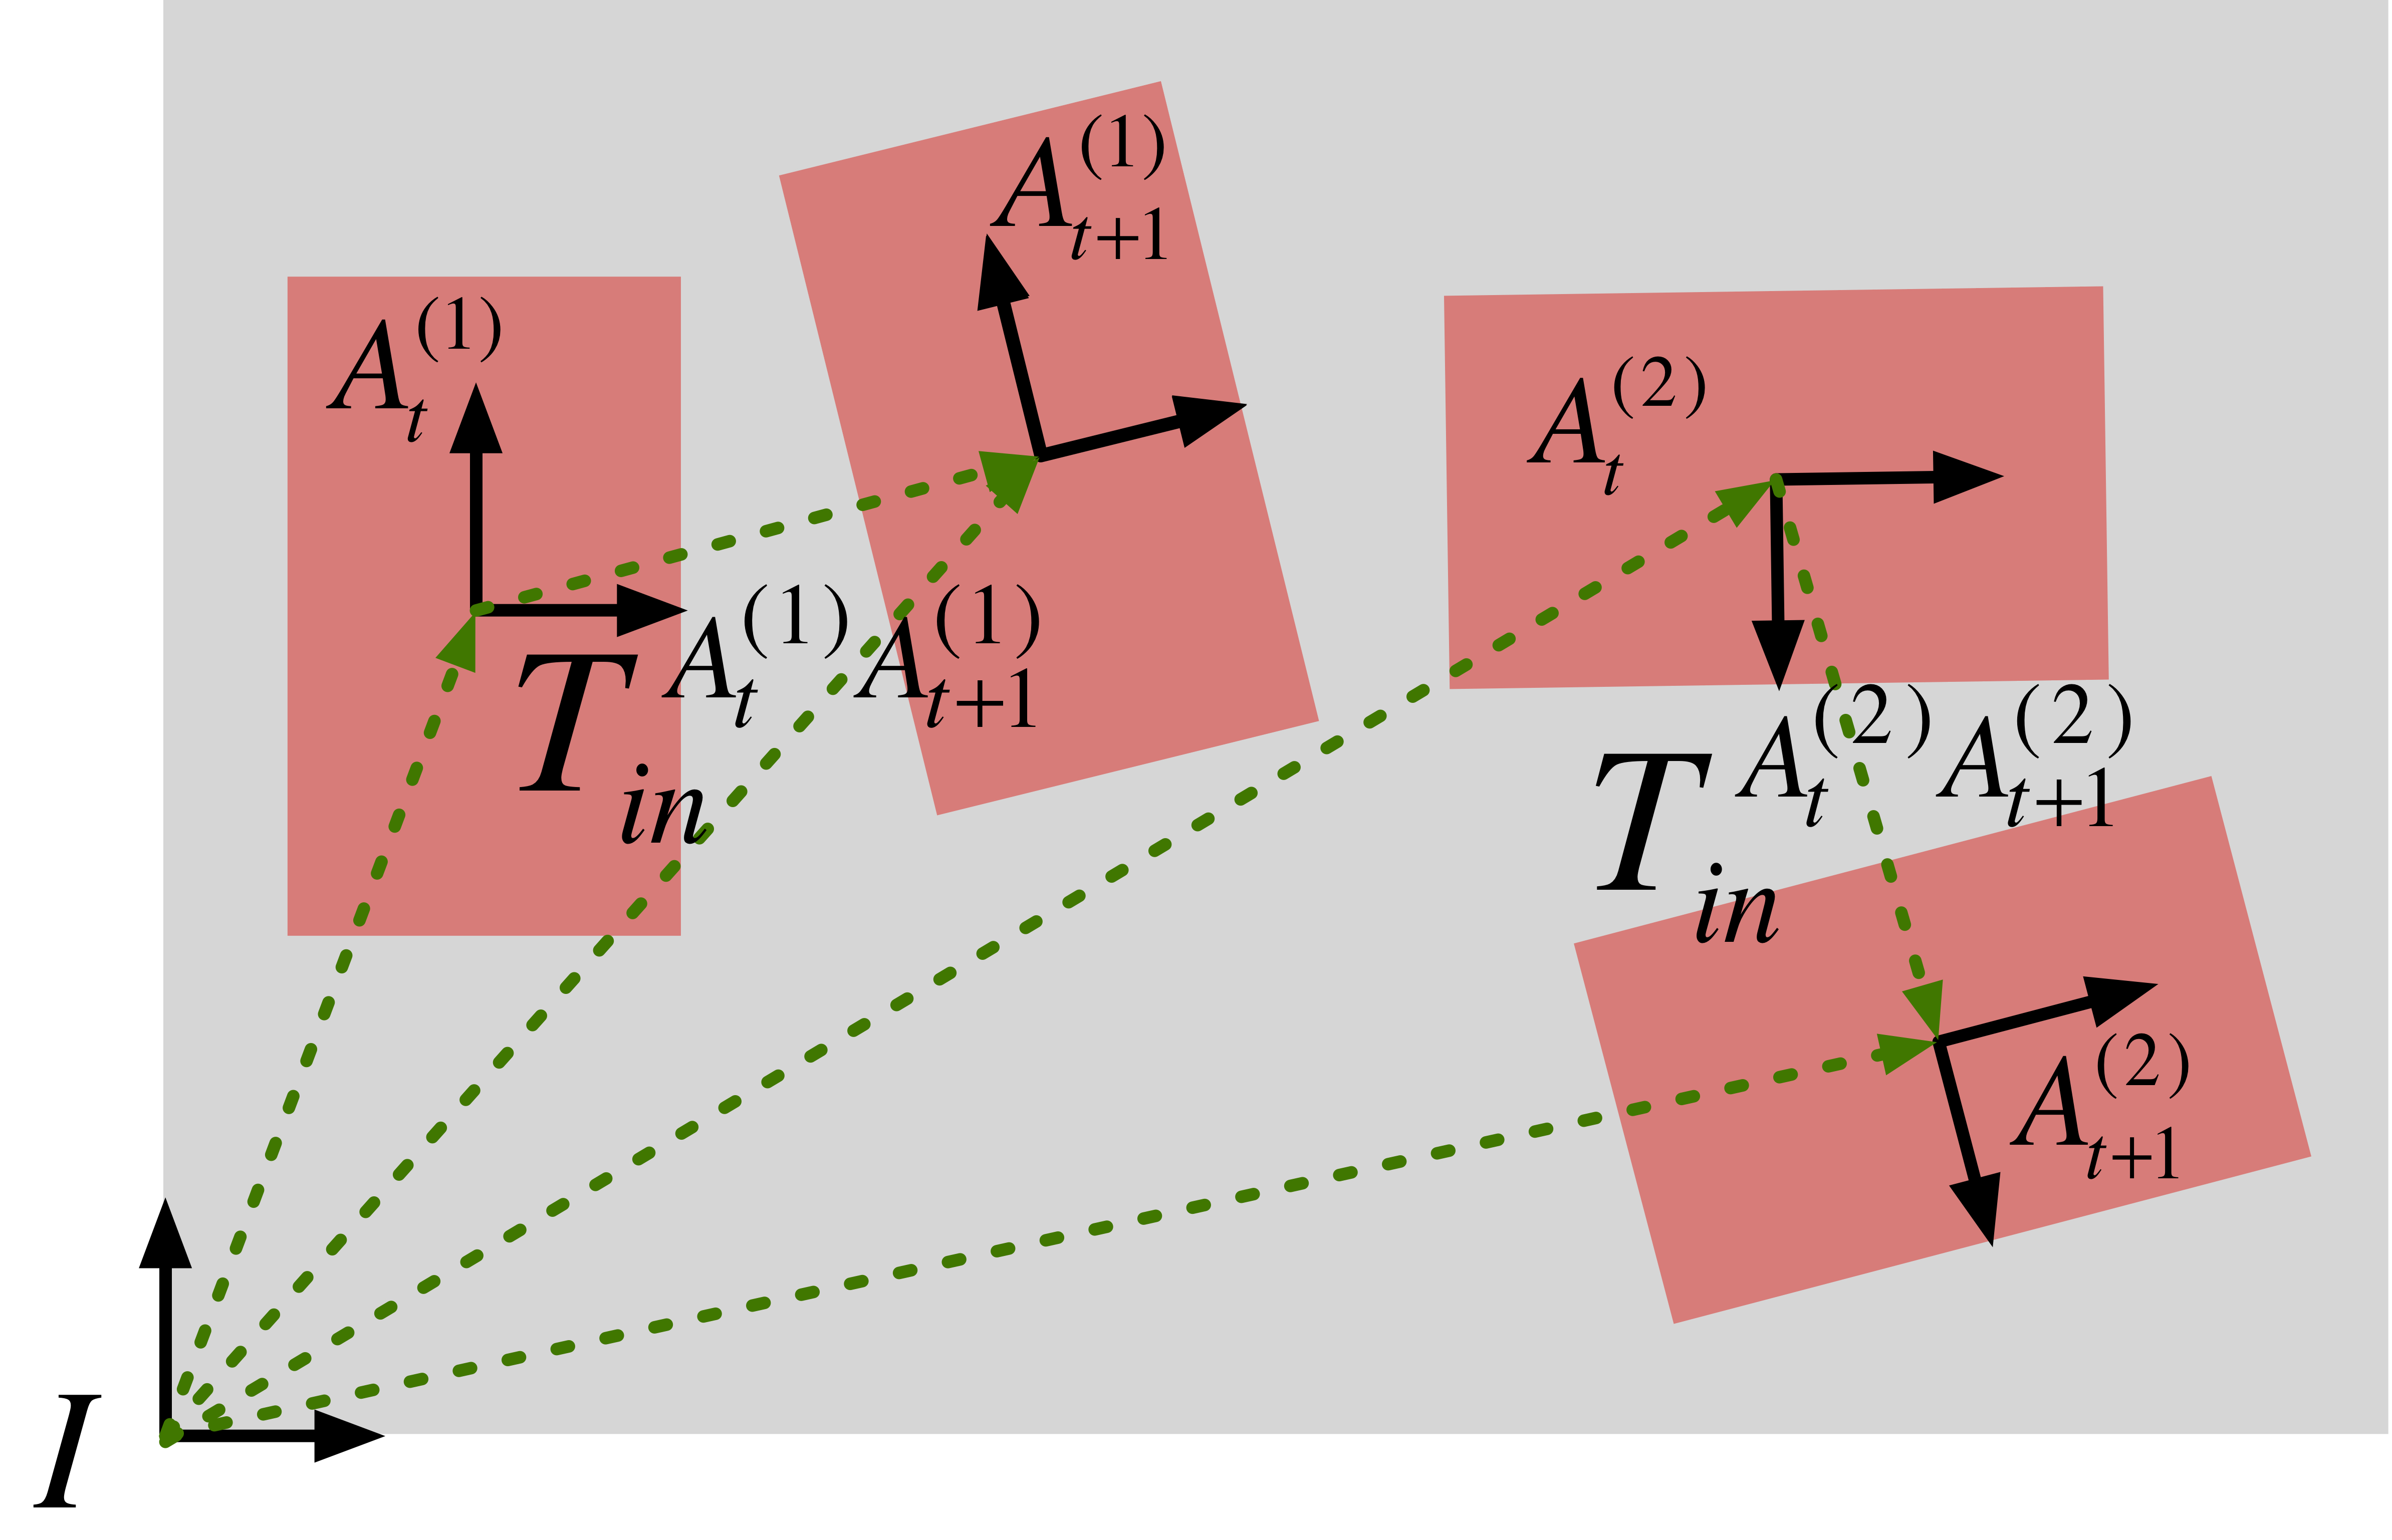
\includegraphics[width=0.34\textwidth]{similarity}
}
\caption[Setup1]{2D projection at time $t$ of a robotic finger with frame at time $t$ of $A_{t}$,
an object with frame $B_{t}$, and a ground plane with constant frame
$O$. Over three time steps this system consists can be described by six rigid body transformations %$T^{A_t, B_t}$, $T^{B_t, O}$, $T^{A_{t-1}, A_{t}}$, $T^{A_{t}, A_{t+1}}$, $T^{B_{t-1}, B_{t}}$, and $T^{B_{t}, B_{t+1}}$.
}
\label{fig:Learning.setup1}
\end{figure*}

\section{Encoding rigid body kinematics}
\label{sec:Representations}

In this section we set up the basic notation required to pose the
above prediction learning problems formally. Without loss of generality we explain the notation using an example from our application domain
(Figure~\ref{fig:Learning.setup1}). Three reference frames $A$, $B$
and $O$ sit in a $3$\nobreakdash-\hspace{0pt}dimensional Cartesian
space. Frame $A$ is attached to a robot finger which pushes an object with frame $B$, which in turn is placed on a table top with frame
$O$.\footnote{Although it is an abuse of notation for brevity we will
  use $A$, $B$ and $O$ to denote either the frame or the body to which  it is attached. So we will talk both of the frame $B$ and the object $B$.} While frame $O$ is fixed, $A$ and $B$ change in time and are observed at discrete time steps $..., t-1, t, t+1, ...$.  Frame $X$ at
time step $t$ is denoted $X_t$, and the rigid body transformation
between a frame $X$ and a frame $Y$ is denoted by $T^{X, Y}$.

From classical mechanics we know that in order to predict the change
in state of a rigid body, it is sufficient to know its mass, velocity
and a net force applied to the body.  Since our method will rely on
learning from object trajectories we cannot assume any knowledge of
the mass and applied forces. We can however, use the motion of a body over time to encode acceleration -- an effect of the applied net
force. We therefore use rigid body transformations $T^{X,Y}$ of the interacting bodies through time (Figure~\ref{fig:Learning.setup1}). Given the additional assumption that the net force and the body mass are constant, two subsequent rigid body transformations $T^{B_{t-1},
  B_{t}}$ and $T^{B_{t},B_{t+1}}$ give a complete description of the
state of some body B (here the object) at time step $t$ in the absence
of the other bodies.  Adding the transformation $T^{B_t, O}$ to give a
triple of transformations thus provides a complete description of the
state of body B in the fixed frame $O$ (the stationary elements of the
environment).  Similarly, a second triple of transformations $T^{A_t,
  O}$, $T^{A_{t-1}, A_{t}}$ and $T^{A_{t}, A_{t+1}}$ provides such a
description for some other body (here the finger) with frame $A$. 
The state of the overall system consisting of these two interacting
bodies with frames $A$ and $B$ and the fixed environment $O$ can
thus be adequately described by these six transformations.

In fact in our representation, we replace transformation $T^{A_t, O}$ by relative transformation $T^{A_t, B_t}$, thus also explicitly capturing the spatial relationship and thus any contacts between $A$ (finger) and $B$ (object). This gives us a representation consisting of the set of six transformations marked in bold dotted lines in Figure~\ref{fig:Learning.setup1}. The prediction problem, simply put, will thus be to predict the motion of the object $B$ in the next step: $T^{B_t,B_{t+1}}$ given these five other transformations. Before defining the problem formally, however, we need to think briefly about how best to store these transformations.

Specifically, since we are interested in learning, we need to express this set of transformations in a way that supports generalised predictions. In general the behaviours of interacting bodies described by frames from Figure~\ref{fig:Learning.setup1} are independent of any inertial frame \cite{kopicki_prediction_2010}. Unfortunately, a na\"{\i}ve representation of transformation $T^{A_{t}, A_{t+1}}$ as $A_{t+1}(A_{t})^{-1}$, or explicitly given inertial frame $I$,
% MAREK CHECK
\begin{equation}
T_{in}^{A_{t}, A_{t+1}} = T^{I, A_{t+1}} (T^{I, A_{t}})^{-1}
\label{eq:Learning.In1}
\end{equation}
\noindent makes the transformation in \eqref{eq:Learning.In1} dependent on the currently used inertial frame $I$ (see
Figure~\ref{fig:similarity}).  This would make the stored transformations poor from the point of view of generalisation. A better way is instead to store all the transformations in a body frame (at learning time) and convert to and from an inertial frame dependent transformation (at prediction time) using similarity transforms.

\begin{figure}[b!]
\centerline{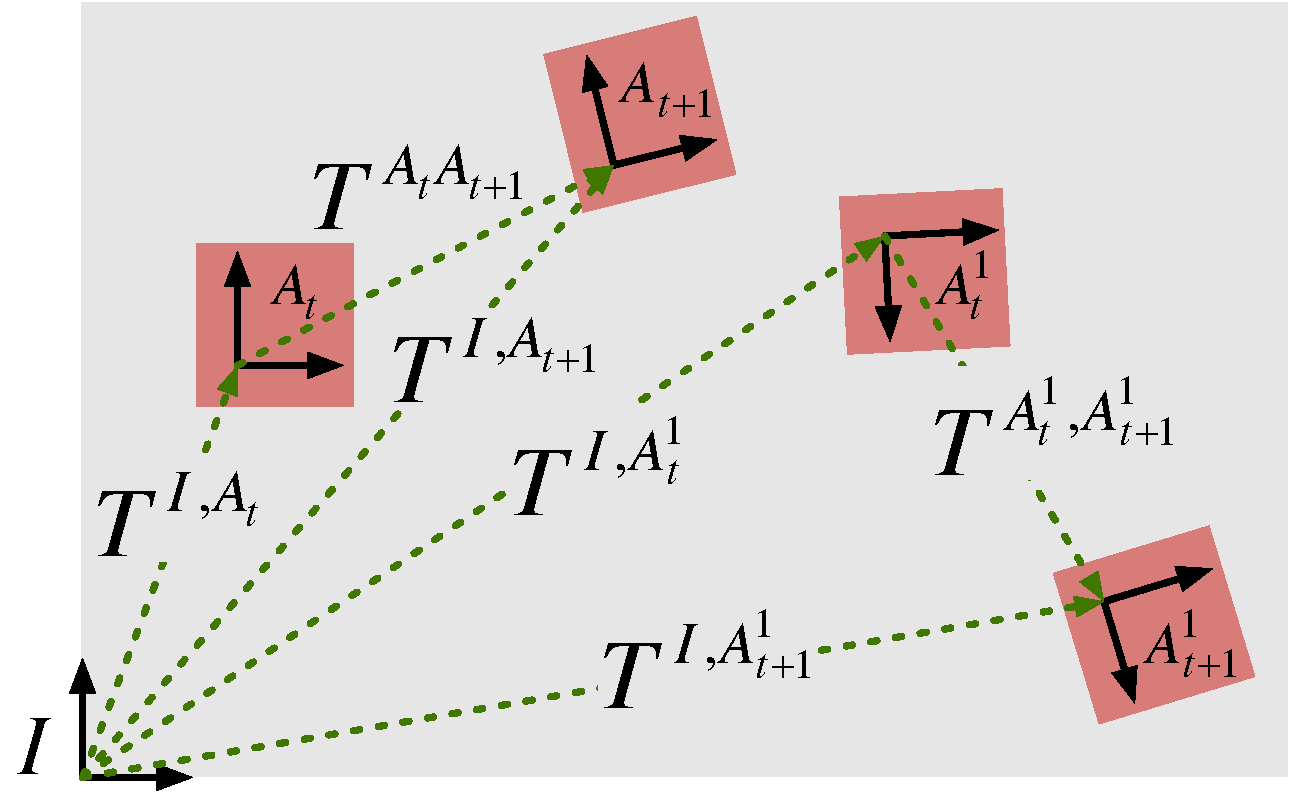
\includegraphics[width=0.85\columnwidth]{similarity-new}}
\caption[Similarity]{ Overhead view of an object on a table starting in two different positions. In each case the motion from $t$ to $t+1$ is the same relative to the instantaneous object body frames $A$ and $A^{1}$. However because transformations $T^{I, A}$ and $T^{I, A^{1}}$ are different, the corresponding transformations in the inertial frame are also different, i.e.\ $T_{in}^{A_{t}, A_{t+1}} \neq T_{in}^{A^{1}_{t}, A^{1}_{t+1}}$.}
\label{fig:similarity}
\end{figure}
Intuitively these similarity transforms align the inertial and body frames, perform the required transformation and then invert the transformation required to align them. In this manner, given the instantaneous object frame $A_{t}$ at time $t$, and the inertial frame dependent transformation
$T_{in}^{A_{t}, A_{t+1}}$, one can obtain the body frame dependent
transformation $T_{body}^{A_{t}, A_{t+1}}$:

\begin{equation}
T_{body}^{A_{t}, A_{t+1}} = (T^{I, A_{t}})^{-1} T_{in}^{A_{t}, A_{t+1}} T^{I, A_{t}}
\label{eq:Learning.Body1}
\end{equation}

\noindent where $T^{I, A_{t+1}} =$ $T_{in}^{A_{t}, A_{t+1}} T^{I, A_{t}} =$ $T^{I, A_{t}} T_{body}^{A_{t}, A_{t+1}}$.

It is this body frame dependent transformation that will be stored during learning. Conversely, when a prediction is required, given a body frame dependent transformation, the object
frame $A_{t}$, and using Equation~\eqref{eq:Learning.Body1}, the
inertial frame dependent transformation $T_{in}^{A_{t}, A_{t+1}}$ is
recovered using:
\begin{equation}
T_{in}^{A_{t}, A_{t+1}} = T^{I, A_{t}} T_{body}^{A_{t}, A_{t+1}} (T^{I, A_{t}})^{-1}
\label{eq:Learning.Body2}
\end{equation}
This technique is critical to generalisation across inertial frames. In the rest of the paper we will retain subscripts $in$, but suppress subscripts $body$, and assume that all transformations $T^{X, Y}$ are transformations in the body frame $X$ related to the equivalent transform in some inertial frame using a similarity transform:
\begin{equation}
T^{X, Y} \equiv T_{body}^{X, Y} = ({T^{I, X}})^{-1} T_{in}^{X, Y} {T^{I, X}}
\label{eq:Learning.Similarity}
\end{equation}

\section{Formal statement: learning to predict}
\label{sec:PredictionProblem}

We now have the basics required to formally describe the one-step and then the multi-step prediction
problem in such a way that they become problems of learning to predict, and we can effectively tackle Problem 1 (Action Interpolation).

\noindent {\bf One step prediction.} The one step prediction problem is formulated as follows: given that we observe the recent and current positions of the finger and object, and know the planned motion of the finger, $T^{A_{t},  A_{t+1}}$, predict the resulting immediate motion of the object,
$T^{B_{t}, B_{t+1}}$.  This is a problem of finding a function~$f$:
\begin{multline}
f: T^{A_t, B_t}, T^{B_t, O}, T^{A_{t-1}, A_{t}}, T^{B_{t-1}, B_{t}}, T^{A_{t}, A_{t+1}} \\ \longrightarrow T^{B_{t}, B_{t+1}}
\label{eq:Learning.long}
\end{multline}

The function $f$ is capable of describing the effects of interactions between rigid bodies $A$ and $B$, providing their physical properties and net forces are constant
in time,\footnote{A dynamic formulation could explicitly incorporate
net forces into the domain and codomain of \eqref{eq:Learning.long}.}
in the limit of infinitesimally small time steps.
Furthermore, it can be approximately learned from observations
for some small fixed time interval $\Delta t$ between time steps.

If robotic manipulations are performed slowly we can assume quasi-static conditions, and ignore all frames at time $t-1$.  This conveniently reduces the dimensionality of the problem, giving a simplified function~$f_{qs}$:
\begin{equation}
f_{qs}: T^{A_t, B_t}, T^{B_t, O}, T^{A_{t}, A_{t+1}} \longrightarrow T^{B_{t}, B_{t+1}}
\label{eq:Learning.short}
\end{equation}

\noindent {\bf Multi-step prediction.} Having stated the one-step prediction problem it is possible to solve
the multi-step prediction problem. Given a predictor (either $f$ or
$f_{qs}$), the initial state of the finger $T^{A_{1}, O}$ and object
$T^{B_{1}, O}$, and knowing the trajectory of the finger $A_{1},
\ldots A_{T}$ over $T$ time steps, one can predict the complete
trajectory of the object $B_{1}, \ldots B_{T}$, by simply iterating
the predictions obtained from $f_{qs}$.  That is, the output of the
predictor at time~$t$ is used as the input to the predictor for the
next time step (Figure~\ref{fig:three-prediction-problems}).

\noindent {\bf Learning to predict as regression.} In principle it is straightforward to acquire a predictor $f$ or
$f_{qs}$ by learning it from data. Given sufficient experience of
object and finger trajectories we can perform a nonparametric
regression analysis by taking $T^{A_t, B_t}, T^{B_t, O}, T^{A_{t},
  A_{t+1}}$ as independent variables, and $T^{B_{t}, B_{t+1}}$
as the dependent variable.  Nonetheless a powerful regression
technique is needed since the domain of $f_{qs}$ has 18~dimensions
or more depending on the parameterisation of motion.

\noindent {\bf Learning to predict as density estimation.} As an alternative to learning the mapping~\eqref{eq:Learning.short} by regression, we can recast $f_{qs}$ as a conditional probability density (CPD) $p_{qs}$ over possible object motions $T^{B_{t},B_{t+1}}$~\cite{kopicki_prediction_2009}:
\begin{equation}
p_{qs}(T^{B_{t}, B_{t+1}} | T^{A_t, B_t}, T^{B_t, O}, T^{A_{t}, A_{t+1}})
\label{eq:Learning.density1}
\end{equation}

The learning problem is then posed as one of density estimation, permitting the modelling of the probabilities of many possible outcomes. 

Either the regression or density estimation formulation can be used in a modular scheme. In that case a separate module is learned for each agent-object-environment combination. Each module interpolates over actions for its context, and thus the system solves problem P1: Action Interpolation for multiple contexts. There is not, however, enough information in the five transformations used as input, to solve either problem P2 (Action Transfer) or problem P3 (Shape Transfer). We now identify the additional information needed to solve these.

\section{Transfer Learning: Representing contacts}
\label{sec:InfoForPrediction}

The input domains of $f$, $f_{qs}$ $p_{qs}$ as proposed above  adequately represent the behaviour of a specific pair of rigid bodies in a specific environment. They thus provide a well posed version of problem P1 (Action Interpolation). Given this information, however, we cannot solve problems P2 (Action Transfer) or P3 (Shape Transfer). This is because there is insufficient information: the input variables only capture {\em global} relations between objects. To properly pose transfer learning problems we must also explictly capture in the input domain all the {\em local} contact relations between the object and its surroundings. 

\begin{figure}[t]
\centerline{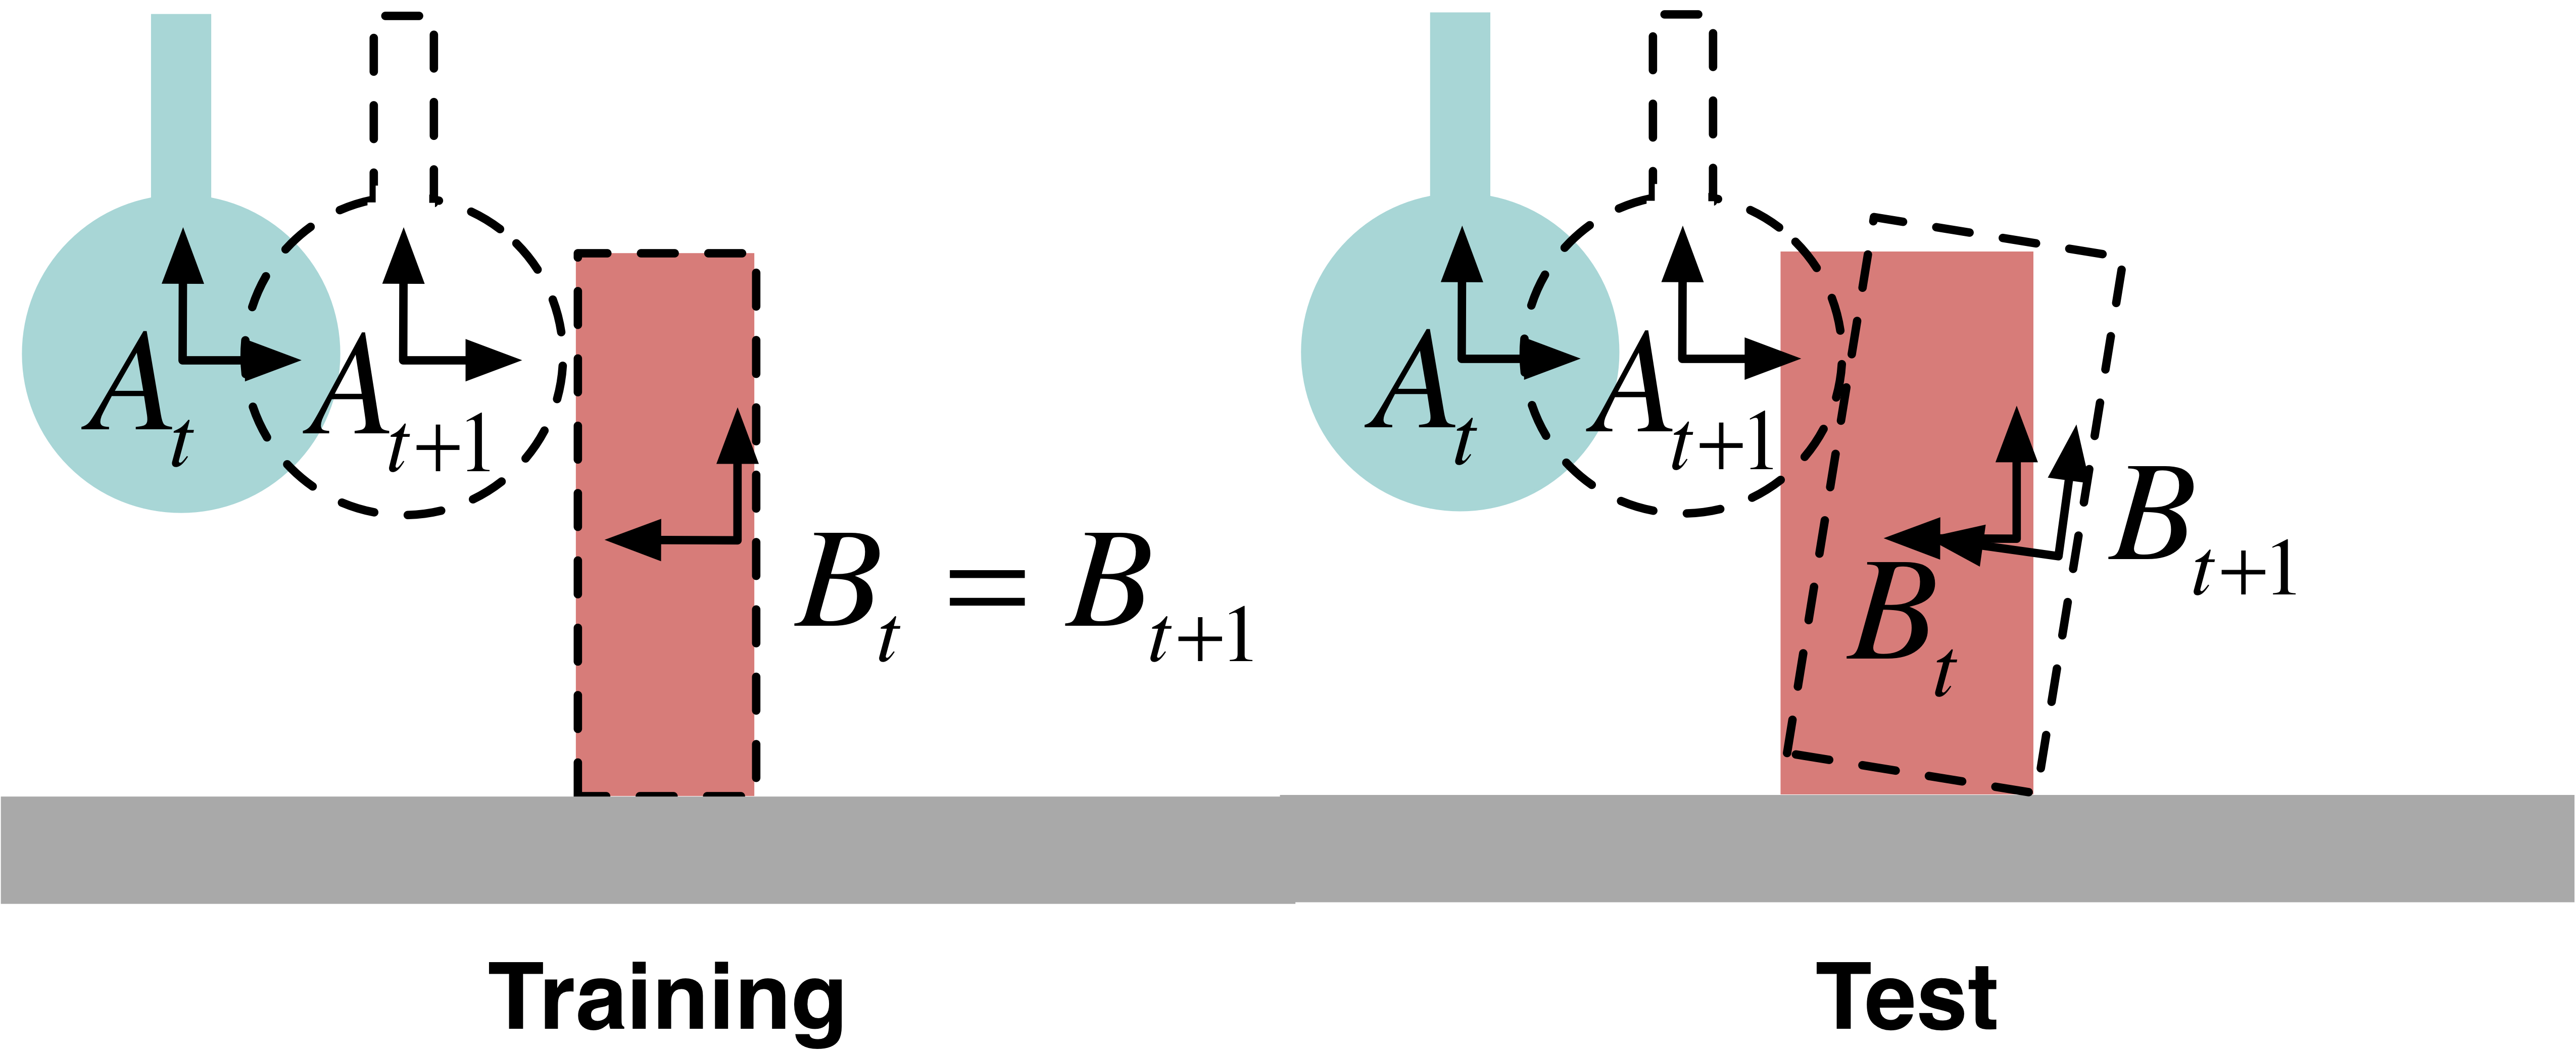
\includegraphics[width=7.5cm]{shapes-colour}}
\caption[Shapes]{Two scenes (left and right),
each with an object on a tabletop, and a finger.
Only the shape of object B differs between the scenes.
Yet when A moves to the position shown by the dashed outline at time $t+1$,
the resulting displacement of B
(represented by the transformation $T^{B_{t}, B_{t+1}}$)
will be quite different.}
\label{fig:Learning.shapes}
\end{figure}

To see why, consider a simple case of shape transfer in Figure~\ref{fig:Learning.shapes}. On the left is a training example. On the right is a test case, where the only difference is that the shape of the object has changed: it is wider. Given the same placement of the frames on object and agent, and the same finger motion, the predicted behaviour using Equation~\eqref{eq:Learning.short} must be the same as for the training example. But this is wrong. To enable the correct prediction to be transferred, additional information is needed in the input domain. Specifically, information on the contact between $A$ and $B$ is required. This can be captured by attaching additional frames to $A$ and $B$ close to their point of contact (see Figure~\ref{fig:Learning.setup2} (centre panel)).

In general an object will have multiple contacts with both the robot, and the environment. Each of these contacts provides a kinematic constraint on the motion of the object, and thus each one of these contacts should be captured as input variables. Only in this way does the predictor have sufficient information to solve transfer problems P2 and P3. Rigid body simulators employ just such contact information. 

%.  A predictor based on
%Equation~\eqref{eq:Learning.short}, and trained on the smaller object
%$B$ (Figure~\ref{fig:Learning.shapes} left scene), cannot generalise
%to the larger object (right scene). This is because the three input
%reference frames ($A_t$, $B_t$, $A_{t+1}$) in the left and right
%panels have identical poses. Thus the predictions will be identical
%even though the shapes are different. For the right panel the
%prediction will be that the finger $A$ will pass into object $B$. So,
%as posed there is insufficient information in the domain of the
%function to allow generalisation. To enable such generalisation
%information on the contact between $A$ and $B$ is required. If object
%$B$ has multiple contacts then information on all of them should be
%included. Physics simulators employ just such contact information to
%inform their predictions. 

\begin{figure*}[t]
\centerline{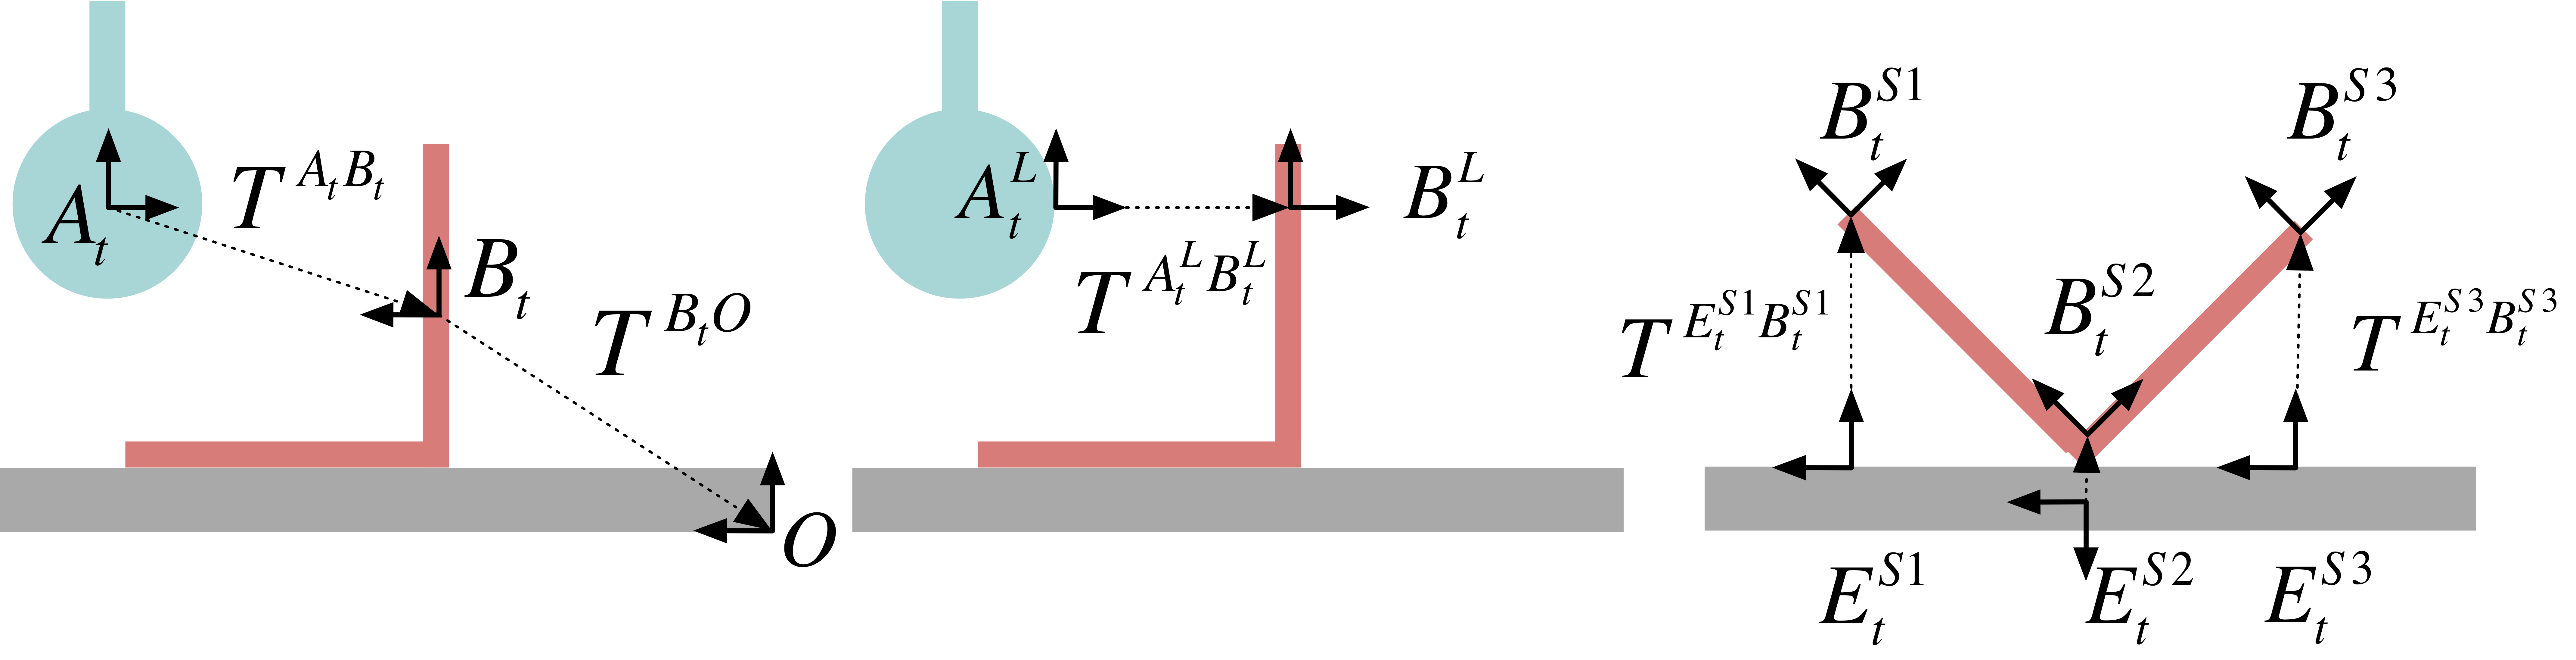
\includegraphics[width=0.75\textwidth]{information}}
\caption{Three types of information useful in prediction problems. Left: (G - global) global frames of reference for the robot, object and the world. Centre: (A - agent) local frames of reference on the robot finger and the closest point on the object. Right (E - environment) local frames of reference on the object and the closest points on surfaces in the environment.}
\label{fig:Learning.setup2}
\end{figure*}

Our approach is to use a pair of local frames to encode each contact or near contact. Each pair encodes one transformation between part of the object $B$ and another body.  To distinguish these local frame pairs from what has gone before we henceforth refer to the main frame attached to each body (as defined in Section~\ref{sec:Representations}) as the global frame for that body. 

We can formally define these local frame pairs as follows. Reconsider
the 2D projection of a robot finger with global frame $A_{t}$, an
object with global frame $B_{t}$, and the environment global frame $O$
(Figure~\ref{fig:Learning.setup2}, left panel). We now also define a pair of local frames
capturing the finger-object contact as $A^{L}_{t}$ and
$B^{L}_{t}$ (centre panel). These are spatially dynamic, i.e.\ at any time $t$ they
are located at the points of closest proximity on the finger and
object respectively.  We define the \textit{agent-object contact}
information as the transformations $T^{A^{L}_{t}, A^{L}_{t+1}}$ and
$T^{A^{L}_t, B^{L}_t}$.

We additionally define $N$ pairs of local frames $B^{Sk}_t$ and $E^{Sk}_t$ to
capture the object-environment contacts, where ($k=1 \ldots N$) (Figure~\ref{fig:Learning.setup2} right panel). We attach the $N$ frames $B^{Sk}_t$
to various parts of the object. Each has a corresponding frame in the
environment $E^{Sk}_t$.  Because they are spatially dynamic the
frames $E^{Sk}_t$ move over surfaces in the environment, as the
object moves. We define the \textit{object-environment contact}
information as the set of transformations $T^{E^{Sk}_t,B^{Sk}_t}$ for $k=1
\ldots N$. To obtain the results presented in this paper, the number and the
locations of the frames $B^{Sk}_t$ on each different object were
determined by hand. In principle this procedure could be automated,
but falls beyond the scope of the current work.

We have already motivated the need for these additional input
variables to support shape generalisation. Their utility can also be seen with respect to changes in
action. The top row of Figure~\ref{fig:ToyExample} shows a training
and a test case for problem P2 (action transfer). The prediction of the test push trajectory requires some encoding of the kinematic constraint
imposed by the contact between the base of the L-shaped flap and the
table. This constraint exists in the training push, but is not
significant since the flap can rotate around its corner, unconstrained
by the base.

\begin{figure}[b]
\centerline{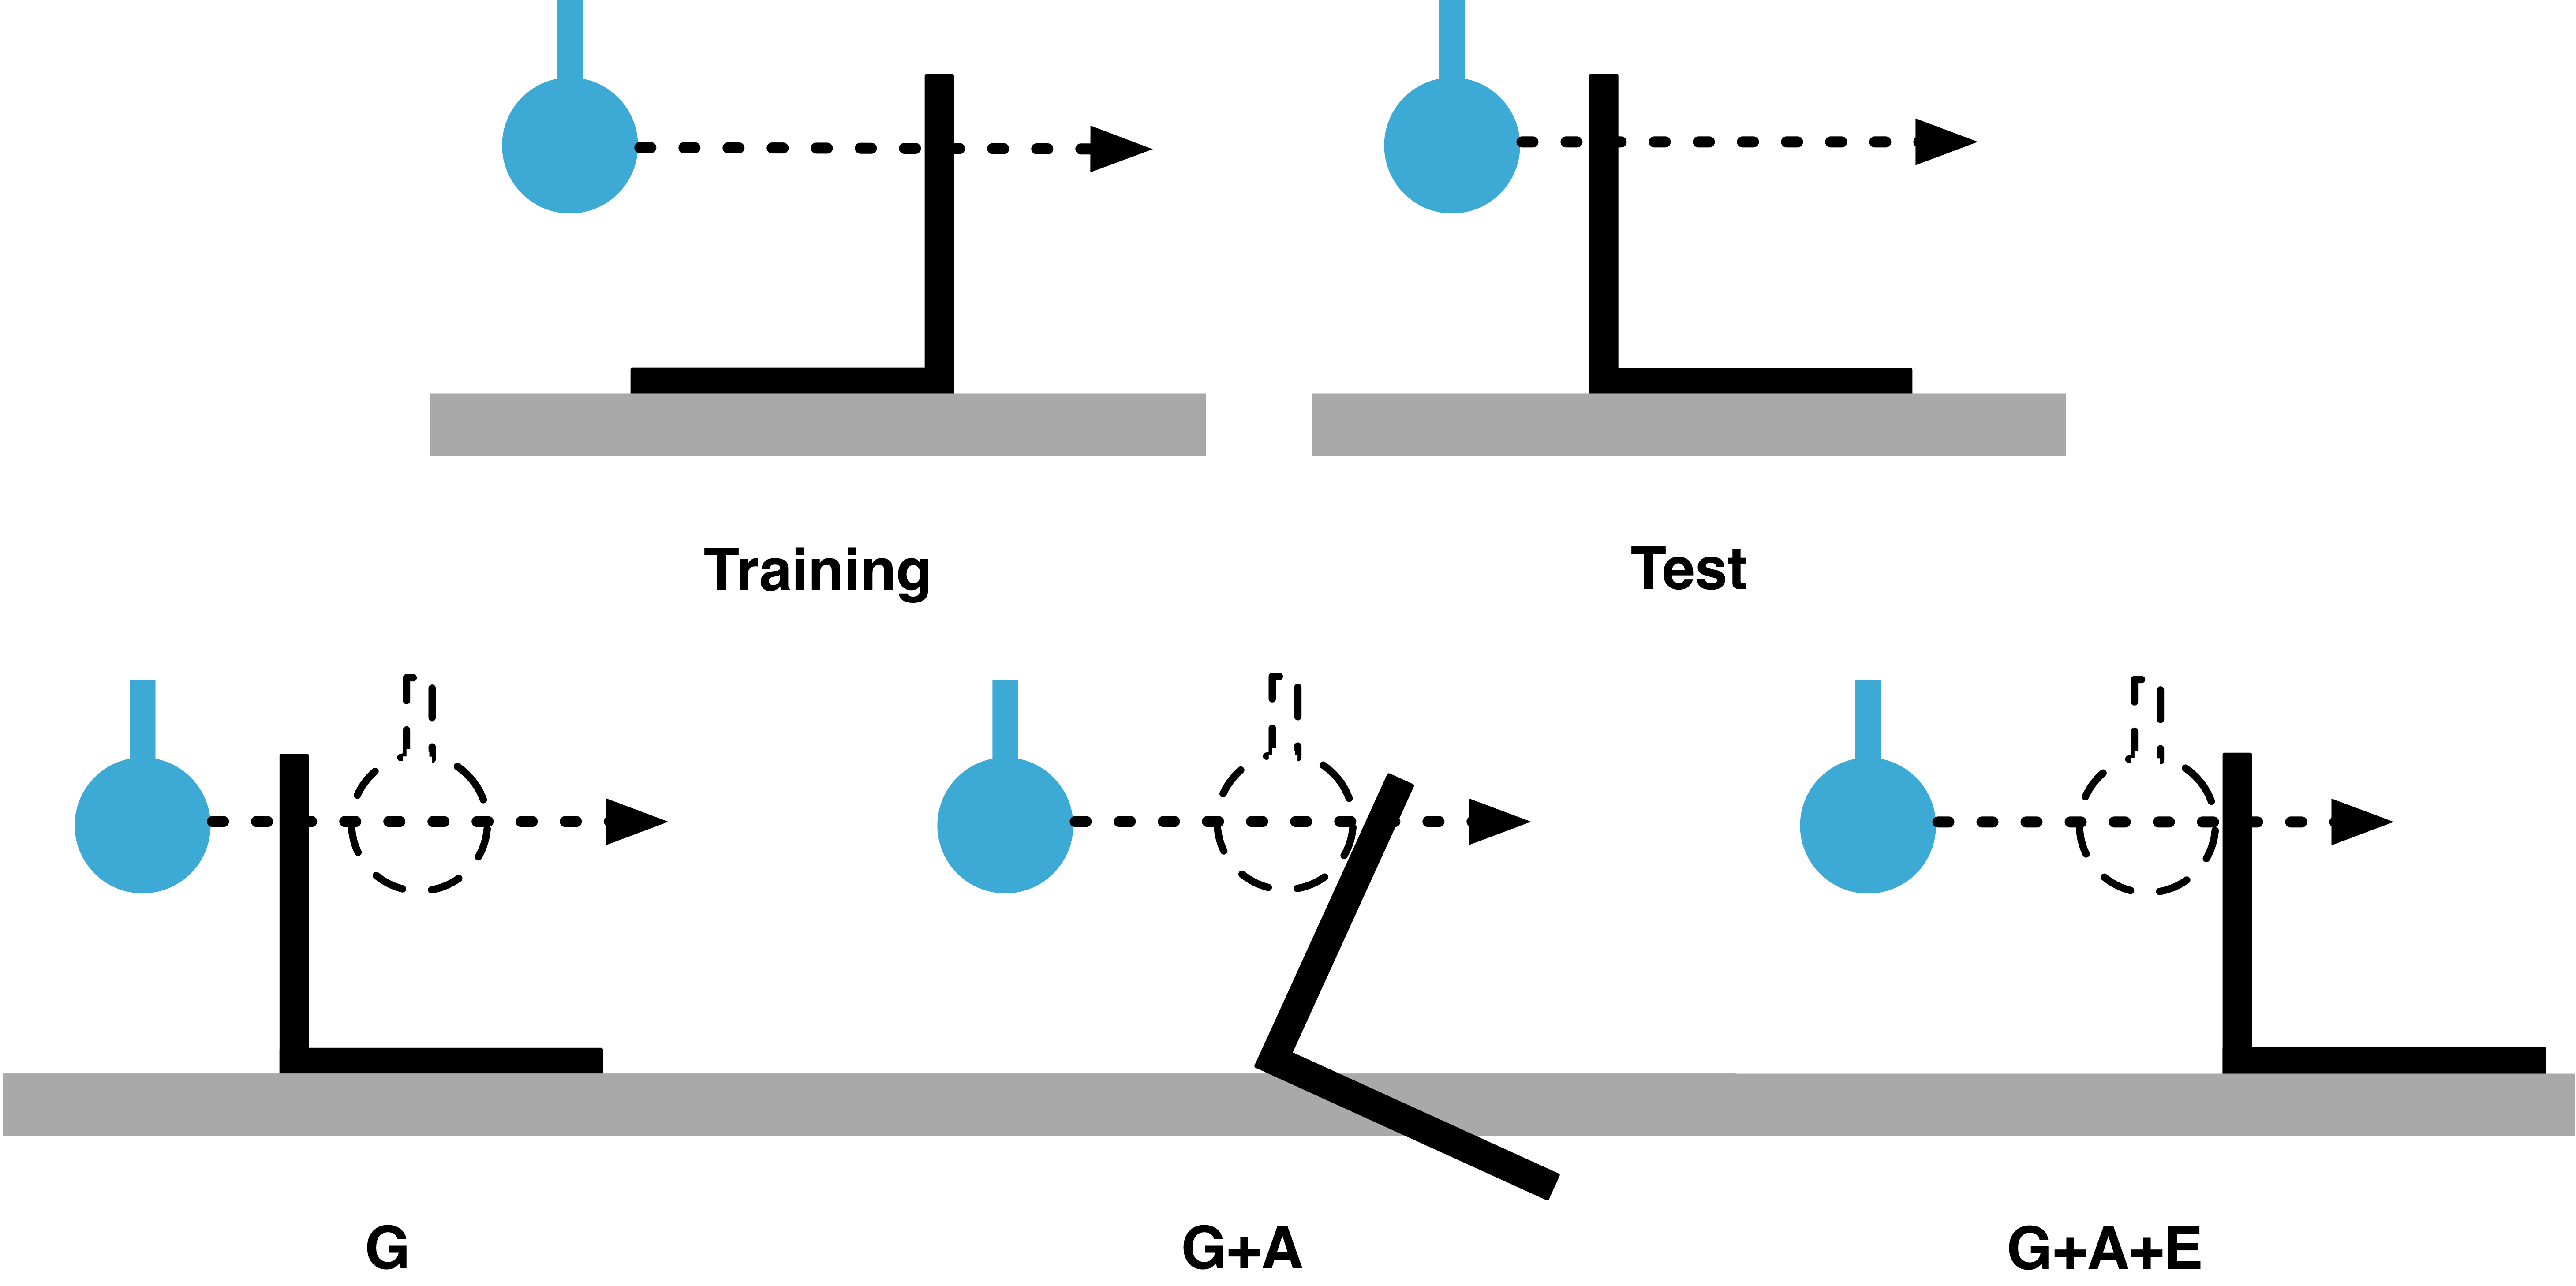
\includegraphics[width=0.8\columnwidth]{BackPushToyExample}}
\caption[ToyExample]{Schematic diagram (2D projection of 3D scene)
in which an object (of L-shaped cross-section) on a supporting surface
is pushed by a robotic finger. 
Various predictors are trained solely on forward pushes (top left), but tested on backwards pushes (top right). The top panels show the push trajectory for the training and test phases, whereas the bottom panels show the outputs from three types of predictor (G, G+A and G+A+E) in the test phase.}
\label{fig:ToyExample}
\end{figure}

We can now consider the effects that different amounts of information
might have on generalised predictions. A predictor endowed only with
information based on the global frames for each body we refer to as
having global information (G). We can add agent-object contact
information to this (G+A), and in turn we can add object-environment
contact information (G+A+E). Now consider the possible predictions for
the test case (Figure~\ref{fig:ToyExample} bottom row). A predictor
using G will predict that the object will not move, because it has no
nearby experience to suggest otherwise. A predictor using G+A has
information from the training case that the object surface will move
with the finger, so that the finger will not pass through it, but is
also capable of predicting that the object rotates about the corner
and into the table since it doesn't model the object-environment
contact. A predictor using G+A+E will have information about the
effect of the contact between the base of the flap and the table and
so should avoid predicting a rotation into the table.

One point is critical here: the above analysis only concerns what the
information allows, it depends on the ability of the learner to
utilise it.  To test this we must incorporate the information into
each learning framework. We can simply extend the regression and density
estimation frameworks to achieve this. For regression one way to
incorporate the extra information $A^{L}_{t}$,$B^{L}_{t}$ and
$E^{Sk}_t$\hspace{-6pt}, $B^{Sk}_t$, provided by the agent and
environment contacts, is simply to enlarge the domain of function~$f$
in Equation~\eqref{eq:Learning.short}, that is:
\begin{multline}
f'_{qs}: T^{A_t, B_t}, T^{B_t, O}, T^{A_{t}, A_{t+1}}, T^{A^{L}_t, B^{L}_t}\{, T^{E^{Sk}_t,B^{Sk}_t}\}_{k=1 \ldots N} \\ 
\longrightarrow T^{B_{t}, B_{t+1}}
\label{eq:Learning.augmented}
\end{multline}

\noindent Unfortunately, because the dimensionality of the domain of $f'_{qs}$ grows with the number of environment contacts $N$,
the difficulty of learning the mapping $f'_{qs}$ rapidly increases
as more environment contacts are added.


The conditional probability density (CPD) $p_{qs}$ over possible object motions $T^{B_{t}, B_{t+1}}$~\cite{kopicki_prediction_2009} is augmented as follows:
\begin{multline}
p_{qs}(T^{B_{t}, B_{t+1}} | T^{A_t, B_t}, T^{B_t, O}, T^{A_{t}, A_{t+1}}, T^{A^{L}_t, B^{L}_t}\\
\{, T^{E^{Sk}_t,B^{Sk}_t}\}_{k=1 \ldots N})
\label{eq:Learning.density}
\end{multline}

Again the dimensionality of the conditioning variables makes density
estimation hard as the number of contacts grows. One way round this in the density estimation case is to factorize the density in a way that
reflects the contact structure. We consider this in the next section. 

\section{Factorised density estimation}
\label{sec:Factors}

Both formulations give learning problems that increase in difficulty as further contacts are added. One question is whether either formulation can be recast so as to take advantage of the natural
problem structure. This section presents one such scheme for the
density estimation (or CPD) formulation, based on a product of experts.

Specifically the CPD formulation allows us to factorise the density
and approximate $p_{qs}$ by making a conditional independence
assumption. The unfactored CPD formulation gives a density over
possible one step motions of the object. We can
factorise this by breaking up the conditioning variables into groups
according to the contacts. This reflects the notion that the behaviour
at one contact is independent of the other contacts: each component of the
product is an expert encoding the likely object motions given a single
kinematic constraint. The product will be maximised by a
motion that best satisfies all the constraints simultaneously.

The computational advantage is that since the component
densities factorise the conditioning variables of $p_{qs}$ their
domains' dimensionalities are smaller, and so potentially they can
better manage the complexity of incorporating more information into
the predictor.  Furthermore, the subset of experts used in the product can be selected dynamically, depending for example on the current set of contacts. Schematically, for some normalisation constant~$C$ we propose the following factorisation:
\begin{equation}
p_{qs} \approx C\ p_{global}\ p_{agent}\ \mathop{\prod}_{k=1 \ldots N}{ p_{env,k}}
\label{eq:Learning.product}
\end{equation}
\noindent where
\begin{subequations}
\begin{align}
p_{global} &\equiv p_{global}(T^{B_{t}, B_{t+1}}|T^{A_{t}, A_{t+1}}, T^{A_t, B_t}, T^{B_t, O})
\label{eq:Learning.densityglobal} \\
p_{agent} &\equiv p_{agent}(T^{B^{L}_{t}, B^{L}_{t+1}}|T^{A^{L}_{t}, A^{L}_{t+1}}, T^{A^{L}_t, B^{L}_t})
\label{eq:Learning.densitylocal} \\
p_{env,k} &\equiv p_{env,k}(T^{B^{Sk}_t, B^{Sk}_{t+1}} | T^{E^{Sk}_t,B^{Sk}_t})
\label{eq:Learning.densityenv}
\end{align}
\end{subequations}

\noindent denote the \textit{global}, \textit{agent-object} and
$k^{th}$ \textit{object-environment} density factors
respectively~\cite{kopicki_prediction_2009}\cite{kopicki_prediction_2010}. 
The one step prediction problem can then be defined as finding the
transformation $\widetilde{T}_{in}^{B_{t}, B_{t+1}}$ expressed in some inertial frame which maximises the product of densities \eqref{eq:Learning.product}:
\begin{equation}
\widetilde{T}_{in}^{B_{t}, B_{t+1}} = \argmax{T_{in}^{B_{t}, B_{t+1}}} \bigg\lbrace
p_{global}\  p_{agent} \mathop{\prod}_{k=1 \ldots N}{ p_{env,k} }
\bigg\rbrace
\label{eq:Learning.MultiFactorProduct}
\end{equation}

\noindent where similarity transforms as described in Section~\ref{sec:Representations} must be used to evaluate $p_{global}$, $p_{agent}$ and the $N$ environment factors $p_{env,k}$ for a given ${T}_{in}^{B_{t}, B_{t+1}}$.
\begin{figure}[t]
\centerline{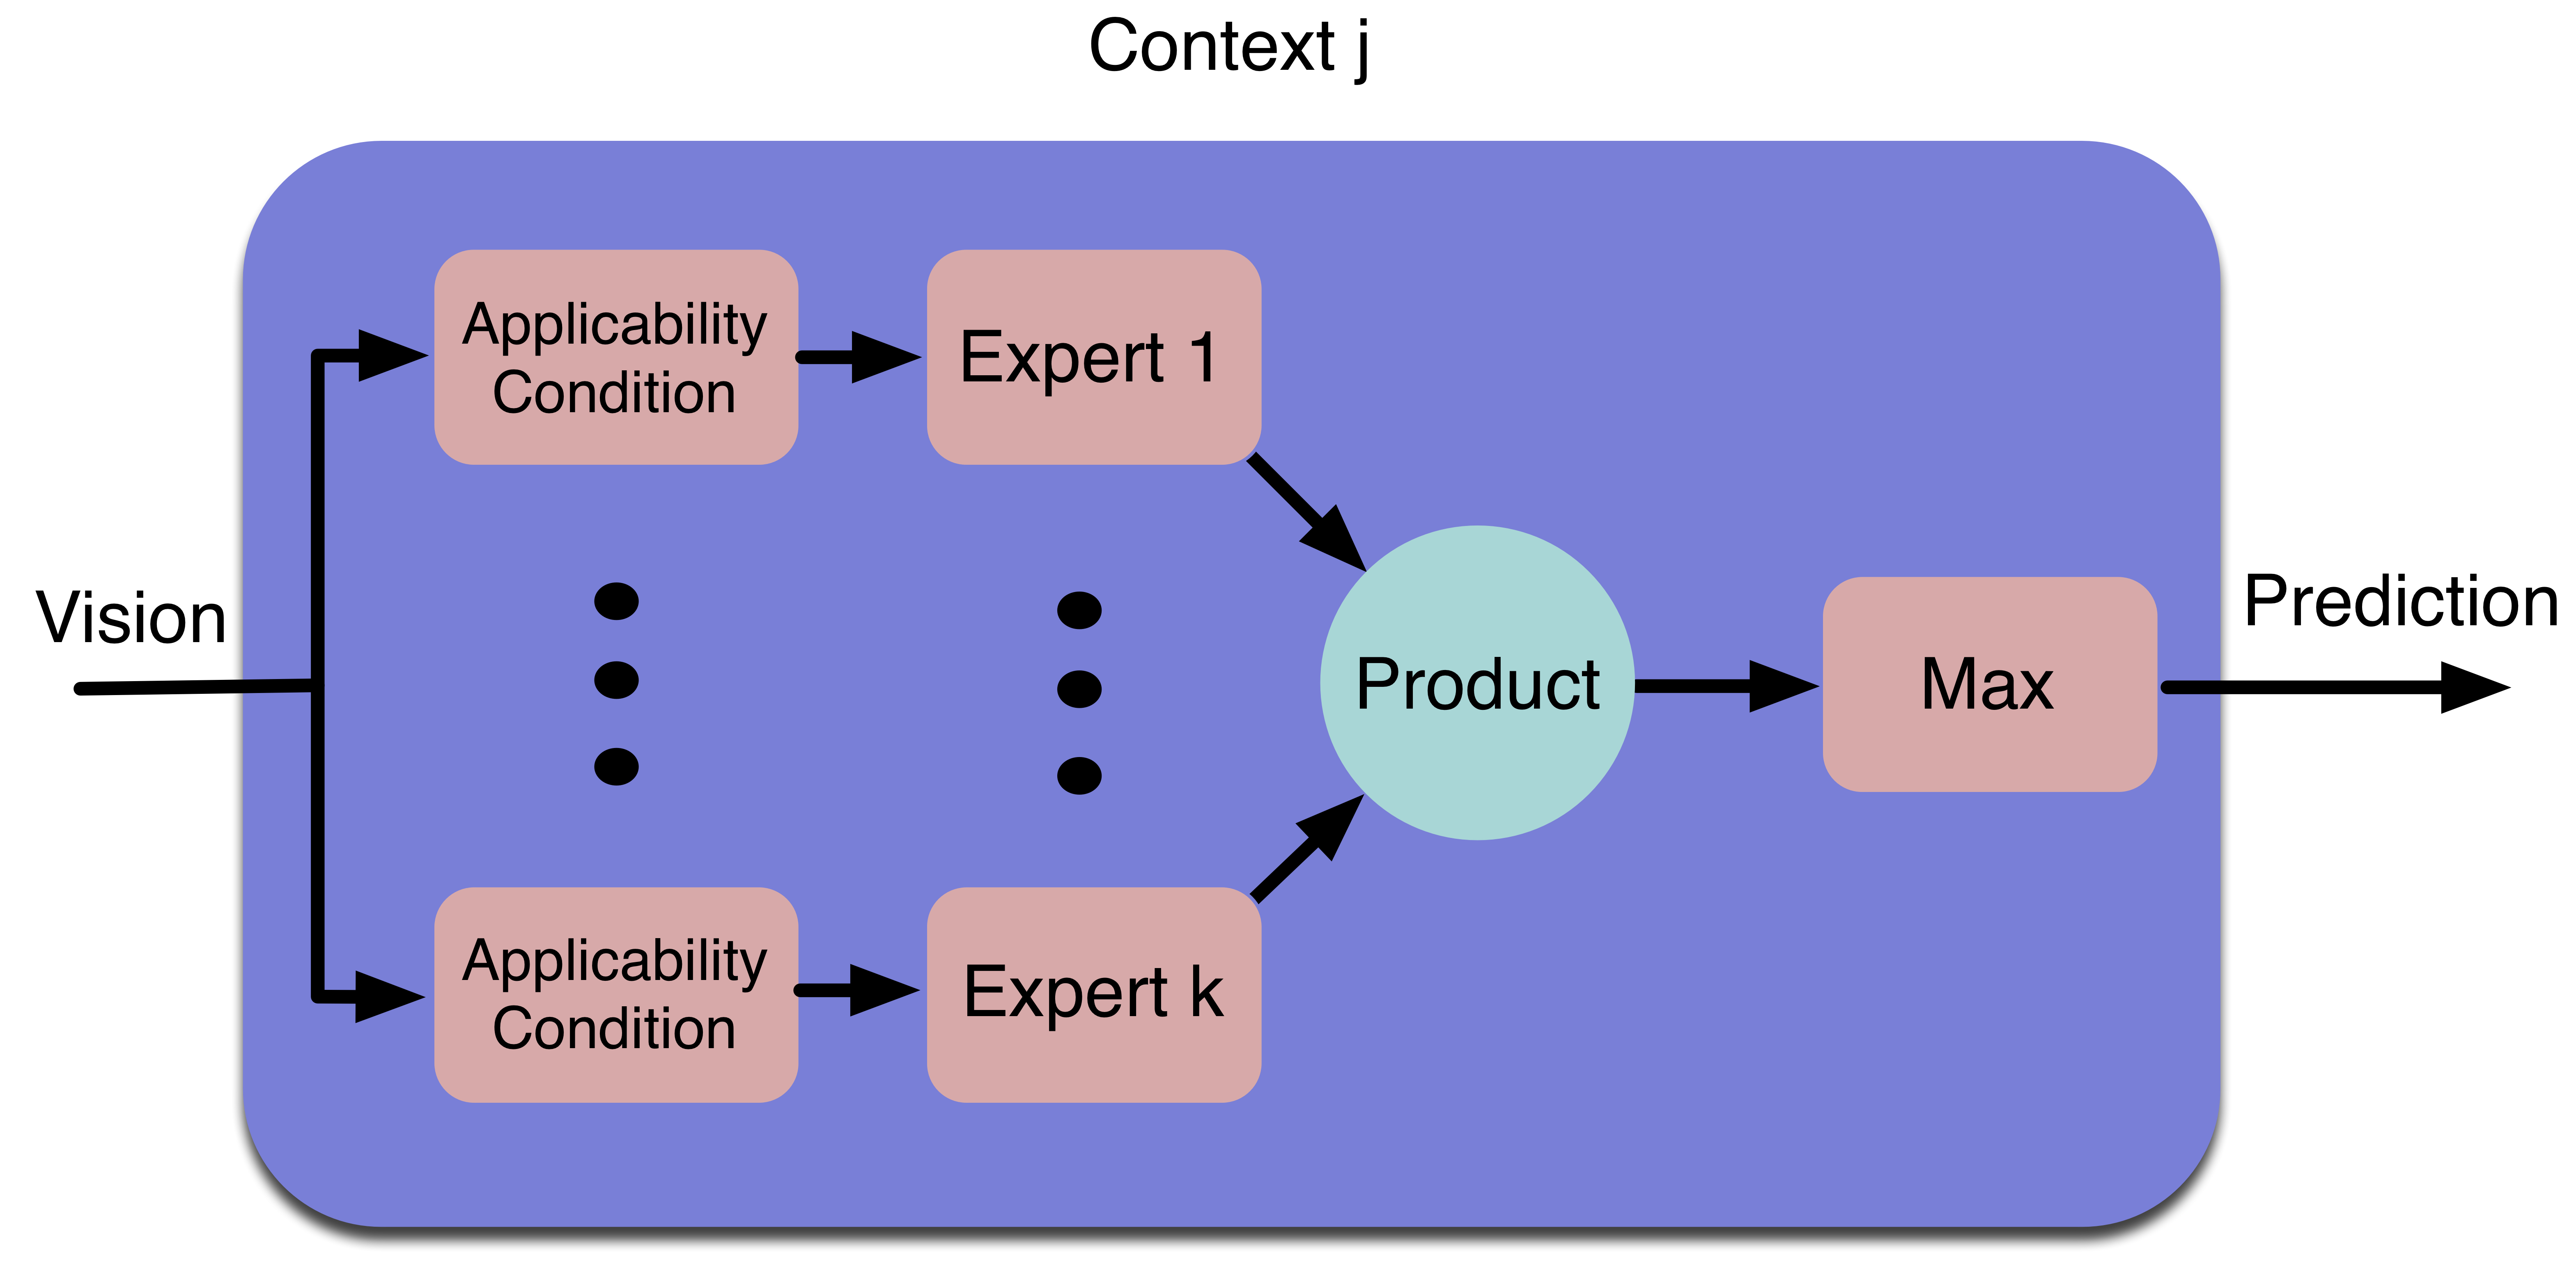
\includegraphics[width=0.85\columnwidth]{product-predictor}}
\caption[Factored Prediction]{ A Dynamic Product of Experts. This gives the structure of a factorised predictor for a single context as depicted in the modular learner in Figure~\ref{fig:three-prediction-problems}. Each expert in the product has an applicability condition which determines whether it contributes to the product. The applicable predictors combine densities over predictions to produce an overall density. This is optimised to produce a specific prediction.}
\label{fig:modular}
\end{figure}

The key property here is that the global, agent and environment densities encode different information about which rigid body transformations are feasible. By taking the product of these densities, only transformations which are feasible in all factors' frames will have high probability in the resulting combined distribution. In addition we make this product dynamic in the number of object-environment factors. Once the object surface is beyond some threshold distance from the environment surface its predictor switches off, and when it is close enough it switches on again. This enables us to keep only relevant predictors in the product at any one time -- improving prediction quality and efficiency. 

In summary we have now described two main formulations (regression and density estimation) able to incorporate varying amounts of information (G, G+A, G+A+E). We have also presented a reformulation of density estimation that factorises the prediction problem given information G+A or G+A+E into a product of experts. Which which information and problem formulation combine to provide the best prediction framework?
Is the factorised problem better able to exploit the additional
information than the unfactorised version? These questions can only be
answered using specific regression and density estimation
algorithms. Having completed our problem formulation we therefore now
turn to the details of the implementations we used for each framework.
